\documentclass[11pt]{beamer}
\usetheme{Boadilla}
\usepackage[utf8]{inputenc}
\usepackage{amsmath}
\usepackage{amsfonts}
\usepackage{amssymb}
\usepackage{listings}
\usepackage{color}

\definecolor{dkgreen}{rgb}{0,0.6,0}
\definecolor{gray}{rgb}{0.5,0.5,0.5}
\definecolor{mauve}{rgb}{0.58,0,0.82}

\lstset{frame=tb,
  language=c++,
  aboveskip=3mm,
  belowskip=3mm,
  showstringspaces=false,
  columns=flexible,
  basicstyle={\small\ttfamily},
  numbers=none,
  numberstyle=\tiny\color{gray},
  keywordstyle=\color{blue},
  commentstyle=\color{dkgreen},
  stringstyle=\color{mauve},
  breaklines=true,
  breakatwhitespace=true,
  tabsize=3
}
\author{From the winter school}
\title{The JetScape Computational framework}
%\setbeamercovered{transparent} 
%\setbeamertemplate{navigation symbols}{} 
%\logo{} 
%\institute{} 
\date{\today} 

%\subject{} 
\begin{document}

\begin{frame}
\titlepage
\end{frame}

%\begin{frame}
%\tableofcontents
%\end{frame}

\begin{frame}
\begin{center}
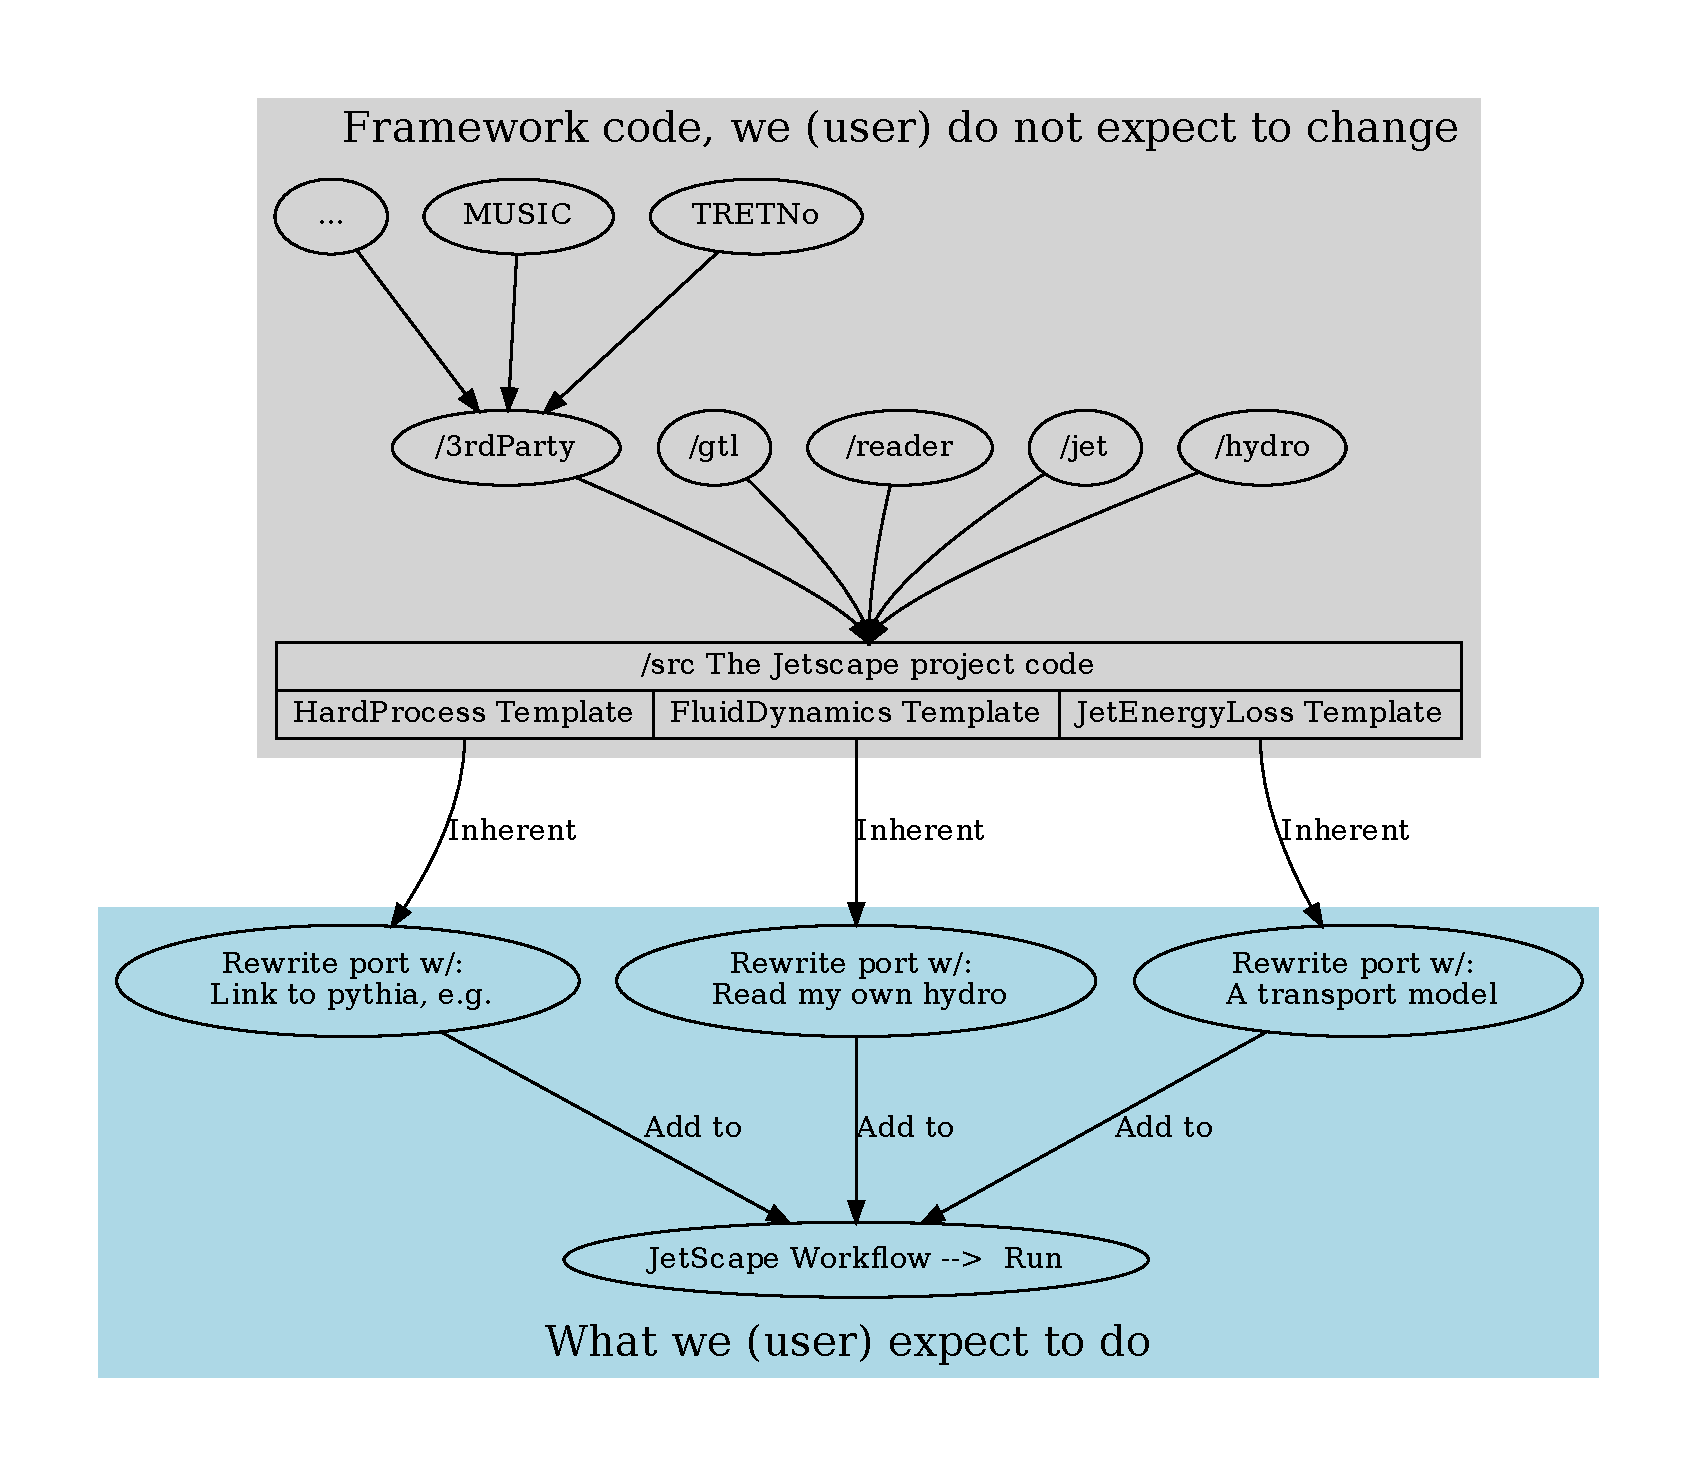
\includegraphics[width=0.9\textwidth]{./framework.pdf}
\end{center}
\end{frame}

\begin{frame}[fragile]{"Easy" combination of multiple transport models}
For example:
\begin{itemize}
\item Matter handles parton evolution at large virtuality ($Q > 1$ GeV e.g.)
\item Martini / LBT (rate equations) apply at low virtuality.
\end{itemize}
In JetScape framework code, this is simply:
\begin{lstlisting}
...
jloss->Add(matter)
jloss->Add(martini)

jlossmanager->Add(joss)
jetscape->Add(jlossmanager)
jetscape->Init()
jetscape->Exec()
...
\end{lstlisting}
The jetscape object will feed and collect the input/output parton data from the transport module. Run order "Matter-Martini" in each time step.

\end{frame}

\begin{frame}{Visualization tool}

\begin{overprint}
\onslide<1> Matter + Martini
\onslide<2> Matter
\onslide<3> Martini
\end{overprint}

\begin{center}
\begin{figure}
\begin{overprint}
\onslide<1>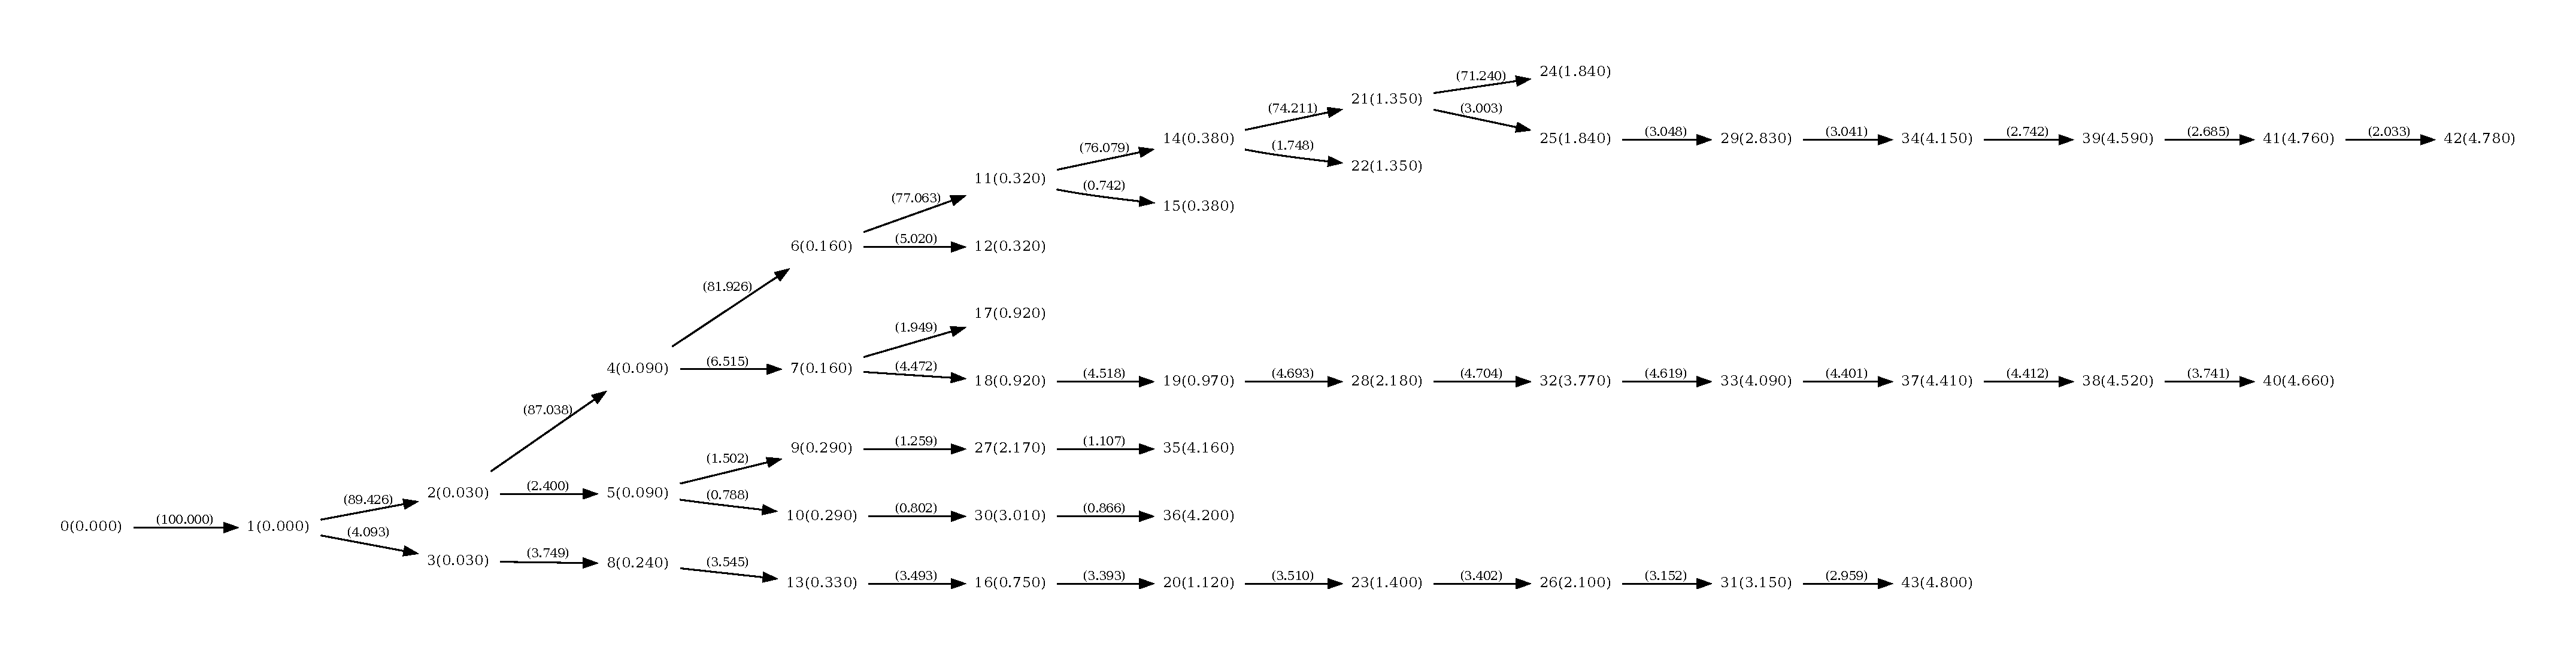
\includegraphics[width=1.8\textwidth]{./sample_jet_graph/graph-Matter-Martini/Jet_Matter_Martini.pdf}
\onslide<2>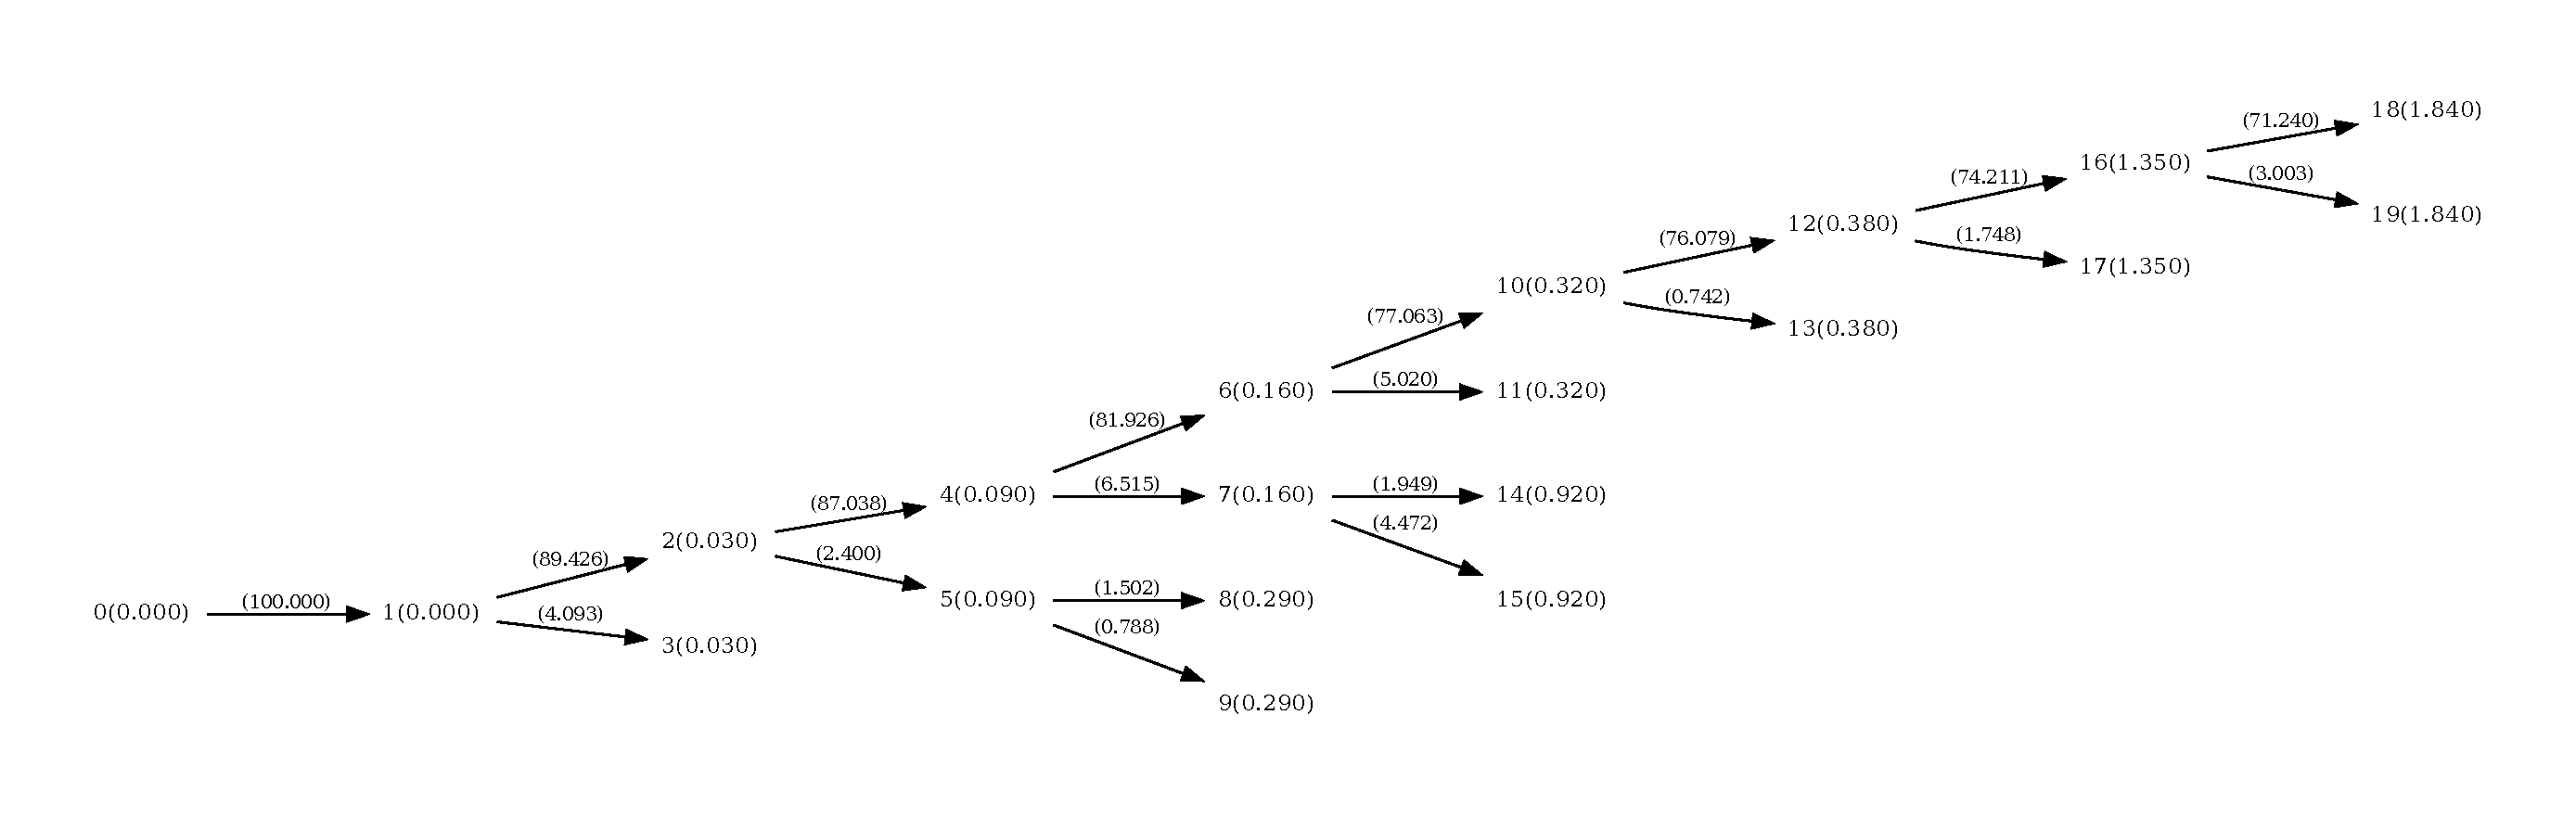
\includegraphics[width=1.2\textwidth]{./sample_jet_graph/graph-Matter/Jet_Matter.pdf}
\onslide<3>
\includegraphics[width=6.\textwidth]{./sample_jet_graph/graph-Martini/Jet_Martini.pdf}
\end{overprint}
\end{figure}
\end{center}
\end{frame}

\end{document}